\chapter{موارد به‌روزرسانی}
\section{ استفاده از \lr{subfigure}}
برای شکل‌های 
\ref{fig:fig1} و \ref{fig:fig2}
به کد مراجعه نمایید
\begin{figure}[h!]
		\centering % <-- added
		\begin{subfigure}{0.33\textwidth}
			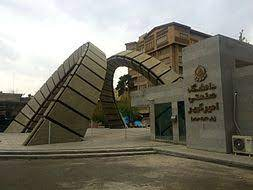
\includegraphics[width=\linewidth]{Images/Chapter6/test1.jpg}
			\caption{\lr{test1}}
			\label{f61}
		\end{subfigure}\hfil % <-- 
		\begin{subfigure}{0.33\textwidth}
			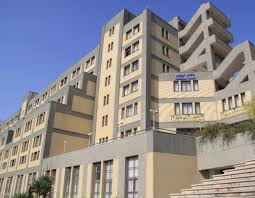
\includegraphics[width=\linewidth]{Images/Chapter6/test2.jpg}
			\caption{\lr{test2}}
			\label{f62}
		\end{subfigure}\hfil % <-- added
        \begin{subfigure}{0.33\textwidth}
			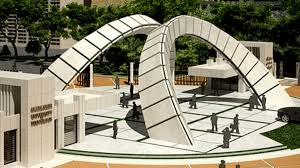
\includegraphics[width=\linewidth]{Images/Chapter6/test3.jpg}
			\caption{\lr{test3}}
			\label{f63}
        \end{subfigure}
		\caption{دانشگاه امیرکبیر}
		\label{fig:fig1}
\end{figure}
 \begin{figure}[ht]
		\centering % <-- added
		\begin{subfigure}{0.45\textwidth}
			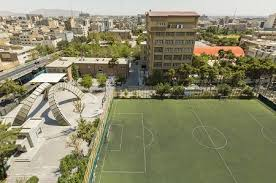
\includegraphics[width=\linewidth, height=0.2\textheight]{Images/Chapter6/test5.jpg}
			\caption{\lr{test5}}
			\label{f64}
		\end{subfigure}\hfil % <-- added
		\begin{subfigure}{0.45\textwidth}
			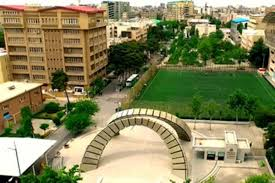
\includegraphics[width=\linewidth, height=0.2\textheight]{Images/Chapter6/test6.jpg}
			\caption{\lr{test6}}
			\label{f65}
		\end{subfigure}
		\caption{پلی تکنبیک}
		\label{fig:fig2}
\end{figure}
\section{فرض}
\begin{asum}
     برای استفاده از فرض کافیست از فرمت زیر استفاده کنید
\begin{latin}
     \normalsize
     \begin{verbatim}
    \begin{asum}
    
    \end{asum}
    \end{verbatim}
\end{latin}
\section{جدول }
\subsection{چندسطری}
مثالی از جدول چند سطری را می‌توانید در \ref{Table1} مشاهده نمایید.
\begin{table}[ht]
    \centering
    \caption{مقایسه الگوریتم‌های بهینه‌ساز}
    \begin{tabular}{|c|c|c|c|} \hline 
        \label{Table1}
        & سناریو & تعداد پارامترها  & تابع هزینه\\  
        \hline
        \multirow{4}{*}{\lr{GWO}} & 1 & 11 & $2.4241$     \\
        & 2 & 8 & $9.1389$           \\
        & 3 & 7 & $6.3343$     \\
        & 4 & 4 & $1.61788$     \\\hline
        \multirow{4}{*}{\lr{PSO}} & 1 & 11 & $20.5801$ \\
        & 2 & 8 & $10.1402$\\
        & 3 & 7 & $3.83659$ \\
        & 4 & 4 & $4.86521$\\\hline
        \multirow{4}{*}{\lr{GA}}  & 1 & 11 & $34.8627$\\
        & 2 & 8 & $33.7109$\\
        & 3 & 7 & $26.4257$\\
        & 4 & 4 & $25.6392$\\\hline						
    \end{tabular}
\end{table}
\end{asum}
\subsection{مقیاس بندی}
برای تنظیم جدول می‌توانید از دستور زیر استفاده نمایید
\begin{latin}
     \normalsize
     \begin{verbatim}
    \adjustbox{max width=\textwidth,max totalheight=\textheight, keepaspectratio}{
    \begin{tabular}...
    .
    .
    .
    \end{tabular}}
    \end{verbatim}
\end{latin}
یا 
\begin{latin}
     \normalsize
     \begin{verbatim}
    \adjustbox{width=\columnwidth,max totalheight=\textheight, keepaspectratio}{
    \begin{tabular}...
    .
    .
    .
    \end{tabular}}
    \end{verbatim}
\end{latin}
نمونه جدول بدون تنظیم
\begin{table}[ht]
    \begin{tabular}{|c|c|c|c|c|c|c|c|c|c|c|c|c|} \hline 
        & $c_1^{\alpha}$ & $c_2^{\alpha}$ & $c_1^{\gamma}$ & $c_2^{\gamma}$ & $d$ & $k$ & $d_{L_2}$ & $d_{L_3}$ & $d_{L_4}$ & $d_{\varepsilon}$ & \lr{SW} & $N$\\  
        \hline
        مثلث  & $6.6$ & $2.4$ & $4.3$ & $11.2$ & $8.6603$ & $1.07$ & $15.3696$ & $24.9362$ & $35.9237$ & $1.5$ & 110 & 58  \\\hline
        پنج شلعی  & $6.1$ & $2.8$ & $4.9$ & $12.7$ & $5.8779$ & $1.09$ & $13.2074$ & $20.6509$ & $29.0499$ & $0.9$ & 75 & 72 \\\hline
        شش ضلعی  & $5.9$ & $2.3$ & $5.2$ & $13.3$ & $5$ & $1.1$& $11.2349$ & $17.5667$ & $23.9169$ & 1 & 70 & 72 \\\hline
    \end{tabular}
    \centering
    \caption{پارامترهای الگوریتم}
    \label{Table2}
\end{table}\\
نمونه جدول با تنظیم سایز
\begin{table}[ht]
\adjustbox{max width=\textwidth,max totalheight=\textheight, keepaspectratio}{%
    \begin{tabular}{|c|c|c|c|c|c|c|c|c|c|c|c|c|} \hline 
        & $c_1^{\alpha}$ & $c_2^{\alpha}$ & $c_1^{\gamma}$ & $c_2^{\gamma}$ & $d$ & $k$ & $d_{L_2}$ & $d_{L_3}$ & $d_{L_4}$ & $d_{\varepsilon}$ & \lr{SW} & $N$\\  
        \hline
        مثلث  & $6.6$ & $2.4$ & $4.3$ & $11.2$ & $8.6603$ & $1.07$ & $15.3696$ & $24.9362$ & $35.9237$ & $1.5$ & 110 & 58  \\\hline
        پنج شلعی  & $6.1$ & $2.8$ & $4.9$ & $12.7$ & $5.8779$ & $1.09$ & $13.2074$ & $20.6509$ & $29.0499$ & $0.9$ & 75 & 72 \\\hline
        شش ضلعی  & $5.9$ & $2.3$ & $5.2$ & $13.3$ & $5$ & $1.1$& $11.2349$ & $17.5667$ & $23.9169$ & 1 & 70 & 72 \\\hline
    \end{tabular}}
    \centering
    \caption{پارامترهای الگوریتم}
    \label{Table3}
\end{table}
\begin{table}[ht]
\adjustbox{width=\columnwidth,max totalheight=\textheight, keepaspectratio}{%
    \begin{tabular}{|c|c|c|c|c|c|c|c|c|c|c|c|c|} \hline 
        & $c_1^{\alpha}$ & $c_2^{\alpha}$ & $c_1^{\gamma}$ & $c_2^{\gamma}$ & $d$ & $k$ & $d_{L_2}$ & $d_{L_3}$ & $d_{L_4}$ & $d_{\varepsilon}$ & \lr{SW} & $N$\\  
        \hline
        مثلث  & $6.6$ & $2.4$ & $4.3$ & $11.2$ & $8.6603$ & $1.07$ & $15.3696$ & $24.9362$ & $35.9237$ & $1.5$ & 110 & 58  \\\hline
        پنج شلعی  & $6.1$ & $2.8$ & $4.9$ & $12.7$ & $5.8779$ & $1.09$ & $13.2074$ & $20.6509$ & $29.0499$ & $0.9$ & 75 & 72 \\\hline
        شش ضلعی  & $5.9$ & $2.3$ & $5.2$ & $13.3$ & $5$ & $1.1$& $11.2349$ & $17.5667$ & $23.9169$ & 1 & 70 & 72 \\\hline
    \end{tabular}}
    \centering
    \caption{پارامترهای الگوریتم}
    \label{Table4}
\end{table}
\subsection{استفاده از قضیه}
\begin{theorem}
تست
\end{theorem}
\begin{proof}
    تست
\end{proof}
برای تغییر کلمه برهان به اثبات، می‌توانید خط 52 در  \lr{commands.tex} را غیر فعال نمایید.
\\
  اشکال هر سطح از  \lr{itemize} را می توانید با مراجعه به
 \lr{commands.tex} تغییر دهید، کامنت‌های مربوطه برای اینکار مشخص شده است (خطوط 44 تا 50).\\
نمونه‌ای از \lr{itemize} چهار سطحی:
\begin{itemize}
    \item تست
    \begin{itemize}
        \item تست
        \begin{itemize}
            \item تست
            \begin{itemize}
                \item تست
            \end{itemize}
        \end{itemize}
    \end{itemize}
\end{itemize}
